\begin{frame}{Impact de l'annotation sur l'entraînement}
    \iffalse
\begin{figure}[htbp]
\centering
\begin{subfigure}[t]{0.40\textwidth}
	\centering
	\resizebox{\linewidth}{!}{
	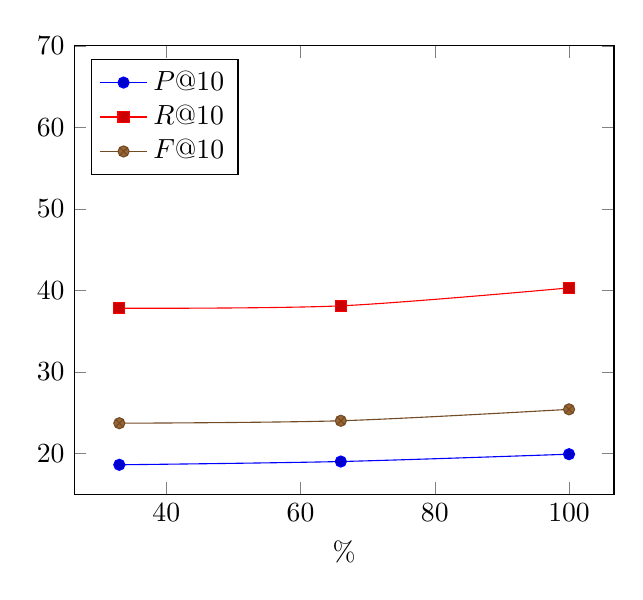
\begin{tikzpicture}%[font=\huge]
	\begin{axis}[smooth, xlabel={$\%$}, %ylabel={$\%$},
				 ymin=15, ymax=70, legend pos=north west]

		\addplot+ coordinates{(33, 18.6)(66, 19.0)(100, 19.9)};
		\addlegendentry{$P@10$}
		\addplot+ coordinates{(33, 37.8)(66, 38.1)(100, 40.3)};
		\addlegendentry{$R@10$}
		\addplot+ coordinates{(33, 23.7)(66, 24.0)(100, 25.4)};
		\addlegendentry{$F@10$}

		%\addplot+[mark=triangle*] coordinates{(33, 26.5)(66, 26.8)(100, 28.2)}; %\addlegendentry{P\@5}
		%\addplot+[mark=*] coordinates{(33, 27.9)(66, 27.8)(100, 29.6)}; %\addlegendentry{R\@5}
		%\addplot+[mark=square*] coordinates{(33, 26.0)(66, 26.0)(100, 27.6)}; %\addlegendentry{F\@5}
	\end{axis}
	\end{tikzpicture}
	}
	\caption{KP20k}
\end{subfigure}
%
\begin{subfigure}[t]{0.40\textwidth}
	\centering
	\resizebox{\linewidth}{!}{
	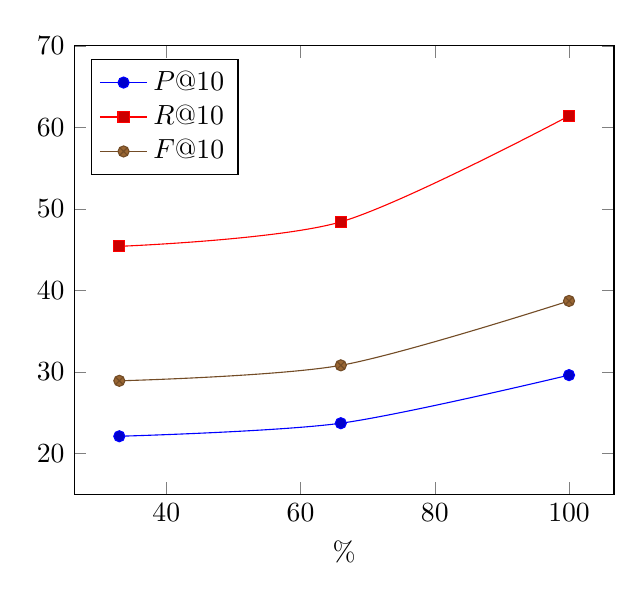
\begin{tikzpicture}%[font=\huge]
		\begin{axis}[
		    smooth,
		    xlabel={$\%$}, %ylabel={$\%$},
	    	ymin=15, ymax=70,
			legend pos=north west
		]

		\addlegendentry{$P@10$}
		\addplot coordinates{(33, 22.1)(66, 23.7)(100, 29.6)};
		
		\addlegendentry{$R@10$}
		\addplot coordinates{(33, 45.4)(66, 48.4)(100,61.4)};
		
		\addlegendentry{$F@10$}
		\addplot coordinates{(33, 28.9)(66, 30.8)(100, 38.7)};
		
		%\addplot+[smooth] coordinates{(33, 33.8)(100, 46.3)}; %\addlegendentry{P\@5}
		%\addplot+[smooth] coordinates{(33, 35.2)(100, 49.3)}; %\addlegendentry{R\@5}
		%\addplot+[smooth] coordinates{(33, 33.3)(100, 46.0)}; %\addlegendentry{F\@5}
		\end{axis}
	\end{tikzpicture}
	}
	\caption{KPTimes}
\end{subfigure}
    \vspace{-1em}
	\caption{Performances de CopyRNN en fonction de la taille du jeu de donnée d'entraînement.} \label{fig:train_percent}
\end{figure}
\fi

\begin{figure}
	\centering
	\resizebox{.7\textwidth}{!}{
	\begin{tikzpicture}%[font=\huge]
	\begin{axis}[
	    scaled x ticks=false,
	    smooth, xlabel={$\#$ documents}, ylabel={$\%$ F@10},
		ymin=21, ymax=44,
		%legend pos=north east,
		legend pos=outer north east,
		xmin=0, xmax=600000,
		%xticklabels={0,100\,K,200\,K,300\,K,400\,K,500\,K},
        %xtick = {0,100000,200000,300000,400000,500000}]
        xticklabels={100\,K,300\,K,500\,K},
        xtick = {100000,300000,500000},
        ]

        \addplot+[color2,every mark/.append style={color=white,fill=color2},mark=*] coordinates{(86641, 34.4)(173282, 37.6)(259923, 38.7)};
        \addlegendentry{NYTimes}


        \addplot[color1,every mark/.append style={color=white,fill=color1},mark=X*] coordinates{(175696, 23.7)(351393, 24.0)(527090, 25.4)};
		\addlegendentry{KP20k}
	\end{axis}
	
	%https://tex.stackexchange.com/questions/413237/get-legend-outside-plot-on-tikz-and-customise-axis-labels
	%https://tex.stackexchange.com/questions/278530/how-i-can-customize-a-legend-on-pgfplots
	\iffalse
	\matrix [draw, matrix of nodes,
            anchor=south east,
        ] at (legend) {
        \multicolumn{2}{c}{Métrique} \\
        \ref{pgfplots:c2r1} & $P@10$ \\
        \ref{pgfplots:c2r2} & $R@10$ \\
        \ref{pgfplots:c2r3} & $F@10$ \\
        \multicolumn{2}{c}{Corpus} \\
        \ref{pgfplots:c2r2} & KP20k \\
        \ref{pgfplots:c2r2} & KPTimes \\
    };
	\fi
	\end{tikzpicture}
	}
	%\caption{Performances de CopyRNN (F@10) en fonction de la taille du jeu de données d'entraînement.}
\end{figure}

    
    \begin{itemize}
        \item Entraînement de CopyRNN avec 33\%, 66\% et 100\% des jeux de données KP20k et KPTimes.
        \item L'ajout de document a KP20k ne permet pas d'augmenter significativement les performances car l'annotation est peu cohérente; contrairement aux mots-clés de KPTimes.
    \end{itemize}
\end{frame}


\againframe<4>{kptimesabs}

\begin{frame}{Document différent, annotation différente, absents}
    \begin{table}[htbp!]
    \centering
    \begin{tabular}{lc@{\hspace*{.2cm}}c c@{\hspace*{.2cm}}c}
        &  \multicolumn{2}{c}{\cellcolor{color2!40} \textbf{KPTimes}} &
        \multicolumn{2}{c}{\cellcolor{color1!40} \textbf{KP20k}} \\
    \cmidrule(lr){2-3} \cmidrule(lr){4-5} \\[-1.5em]
    \% & \small{Prs} & \small{Abs} & \small{Prs} & \small{Abs} \\
    \midrule
    %\cmidrule{1-4}
    \cellcolor{color2!40} CopyNews
        & \cellcolor{color2!40} 61,2 & \cellcolor{color2!40} 38,8 & 51,1 & 48,9 \\
    %\cmidrule(lr){1-2} \cmidrule(lr){3-4}
    \cellcolor{color1!40} CopySci
        & \textbf{94,0} & \pad{0}5,1 &  \cellcolor{color1!40} \textbf{92,0} & \cellcolor{color1!40} \pad{0}8,0 \\
    \bottomrule
    \end{tabular}
    \caption{Pourcentage de mots-clés présents et absents.}
    %produit automatiquement par le modèle CopyRNN entraîné sur KPTimes (CopyNews) et KP20k (CopySci) et testé sur ces deux jeux de données.}
    \label{tab:ratio_prsabs_transfer}
\end{table}
    \begin{itemize}
        \item \colorbox{color1!40}{CopySci} produit presqu'exclusivement des mots-clés présents.
        \item Il est plus \textbf{risqué} de produire des \textbf{mots-clés absent} en situation de \textbf{généralisation}.
    \end{itemize}
\end{frame}


\begin{frame}{Validation du choix des méthodes}
    %\textbf{Métriques} : \map{}
    
    \begin{table}[!ht]
    \centering
    \resizebox{.7\textwidth}{!}{
    \begin{tabular}{l|cc}
        \toprule
            \textbf{Système} & 
            \textbf{\map} & 
            \textbf{P@10} \\
        \midrule
            \textbf{\textsc{Bm25}+RM3} & \best{35,5} & \best{38,9} \\
            {QL+RM3} & 34,4 & 36,1 \\
            1\textsuperscript{er} {\small \cite{fujita_notes_2001}} & 
            31,9 & 37,4 \\
            \textbf{\textsc{Bm25}} & 31,9 & 37,1 \\
            2\textsuperscript{nd} {\small \cite{murata_crl_2001}} & 
            31,3 & 36,1 \\
            {QL} & 31,2 & 35,1 \\
            3\textsuperscript{èm} {\small \cite{chen_berkeley_2001}} &
            26,2 & 33,9 \\
        \bottomrule
    \end{tabular}
    }
    
    \vspace{.5cm}
    Scores des meilleurs systèmes de la compétition NTCIR-2.
\end{table}

\end{frame}

\begin{frame}{Impact des mots-clés seuls}
    
\begin{center}
\begin{tabular}{llrr}
\toprule
         &   \bm{} &  +RM3 \\
\cmidrule(lr){1-3}
\tr{}       & -     & - \\
+ Kea (KP20k)&13,66 & 11,59 \\
+ MPRank    & 13,68 & 13,48 \\
\addlinespace
+ CopyRNN   & 16,61 & 17,02 \\
+ CorrRNN   & 15,54 & 15,63 \\
\cmidrule(lr){1-3}
\trm{}      & 15,51 & 16,00 \\
+ Kea (KP20k)&21,97 & 25,68 \\
+ MPRank    & \best{22,42} & 25,78 \\
\addlinespace
+ CopyRNN   & 21,91 & 27,32 \\
+ CorrRNN   & 21,61 & \best{27,39} \\
\bottomrule
\end{tabular}
\end{center}
\end{frame}

\begin{frame}{Impact des mots-clés seuls (cont'd)}
    \usepgfplotslibrary{groupplots}


\begin{figure}[!ht]
    \centering
    
    \begin{tikzpicture}[trim axis left,trim axis right]

    \begin{groupplot}[
        group style={
          group size=1 by 2,
          vertical sep=1.3cm,
        },
        width=0.7\textwidth, height=5cm,
        xmin=-1, xmax=10,
        xtick = {0, 1, 2, 3, 4, 5, 6, 7, 8, 9},
        tick pos=left,
        grid style={dashed, gray!50},
        xmajorgrids,
        legend columns=1,
        %legend style={
        %    anchor=north west,
        %    at={(-0.09,-0.2)}
        %},
    ]
    
    \nextgroupplot[
        %ymin=34.75, ymax=38,
        xticklabels={,,,},
        %ytick = {35, 36, 37},
        legend to name={CommonLegend}
    ]
    \node[] at (axis cs: .4, 26.5) {{{{\small Auteur}}}};

    \addplot+[smooth] plot coordinates {
    (0, 16.0)(1, 21.8)(2, 23.47)(3, 26.19)(4, 26.82)(5, 27.32)(6, 27.27)(7, 26.79)(8, 27.97)(9, 28.31)
    };
    \addlegendentry{CopyRNN}
    
    \addplot+[smooth] plot coordinates {
    (0, 16.0)(1, 22.08)(2, 23.1)(3, 25.11)(4, 25.87)(5, 27.39)(6, 27.9)(7, 27.07)(8, 27.55)(9, 26.71)
    };
    \addlegendentry{CorrRNN}
    
    \addplot+[smooth] plot coordinates {
    (0, 16.0)(1, 20.36)(2, 19.84)(3, 22.22)(4, 23.47)(5, 25.68)(6, 26.99)(7, 26.92)(8, 27.73)(9, 27.63)
    };
    \addlegendentry{Kea (KP20k)}

    \addplot+[smooth] plot coordinates {
    (0, 16.0)(1, 17.74)(2, 20.83)(3, 21.6)(4, 22.83)(5, 25.78)(6, 27.05)(7, 26.84)(8, 27.37)(9, 27.67)
    };
    \addlegendentry{MPRank}

    % baseline
    \addplot[mark=none, black, dashed] coordinates {(0, 16.0) (9, 16.0)};

    %\legend{}

    \nextgroupplot[
        yshift=1cm,
        %ymin=32.25,ymax=36,
        xticklabels={$N$=0\quad~~,1, 2, 3, 4, 5, 6, 7, 8, 9},
        %ytick = {32, 33, 34, 35},
    ]
    \node[] at (axis cs: .4, 17.5) {{{{\small None}}}};
    
    \addplot+[smooth] plot coordinates {
    (0, 0)(1, 4.14) (2, 7.5)(3, 11.51)(4, 14.21)(5, 17.02)(6, 18.29)(7, 19.11)(8, 19.5)(9, 20.4)
    };
    %\addlegendentry{CopyRNN}
    
    \addplot+[smooth] plot coordinates {
    (0, 0)(1, 6.36)(2, 9.72)(3, 12.57)(4, 14.87)(5, 15.63)(6, 17.17)(7, 18.11)(8, 18.02)(9, 18.09)
    };
    %\addlegendentry{CorrRNN}
    
    \addplot+[smooth] plot coordinates {
    (0, 0)(1, 5.86)(2, 8.02)(3, 8.51)(4, 10.43)(5, 11.59)(6, 14.17)(7, 15.44)(8, 16.43)(9, 17.05)
    };
    %\addlegendentry{KeaOneModel}
    
    \addplot+[smooth] plot coordinates {
    (0, 0)(1, 4.94)(2, 7.5)(3, 8.95)(4, 10.8)(5, 13.48)(6, 13.98)(7, 14.08)(8, 14.92)(9, 15.15)
    };
    %\addlegendentry{MPRank}


    \end{groupplot}
    %\end{axis}
    
    \node[right=2cm of group c1r1.east]{\ref{CommonLegend}};
    
    \end{tikzpicture}
    %\end{subfigure}


    \caption{Scores de \map{} pour \textsc{Bm25}+RM3 sur NTCIR-2 en fonction du nombre $N$ de mots-clés prédits. Le symbole $\square$ indique une amélioration significative par rapport aux résultats sans mots-clés prédits.}
    \label{fig:n_vs_perf}
\end{figure}
\end{frame}

\begin{frame}<1>{Catégorisation PRMN}
    \begin{figure}[ht]
    \centering
    %\centerfloat
    \resizebox{0.98\textwidth}{!}{%
    \begin{tabular}{|p{1.3\textwidth}|}
%\begin{mdframed}[backgroundcolor=blue!2, font=\small]
\textbf{Study on the Structure of Index Data for \hl{c1}{Metasearch} \hl{c3}{System}} {\footnotesize(id: gakkai-e-0001384947)}

\vspace{.9em}

This paper proposes a new technique for \hl{c1}{Metasearch} \hl{c3}{system}, which is based on the grouping of both keywords and URLs.
This technique enables \hl{c1}{metasearch} \hl{c3}{systems} to \hl{c5}{share} \hl{c4}{information} and to reflect the estimation of \hl{c6}{users'} preference.
With this \hl{c3}{system}, \hl{c6}{users} can search not only by their own keywords but by similarity of HTML documents.
In this paper, we describe the principle of the grouping technique as well as the summary of the existing \textbf<2>{\hl{c2}{search} \hl{c3}{systems}}.

\vspace{1.1em}

\textbf{Mots-clés présent}: \phantom{du texte} \hl{c1}{Metasearch} --
\textbf<2>{\hl{c2}{Search} \hl{c3}{System}}

%\vspace{.7em}

\textbf{Mots-clés absent}: \\
\quad \hl{c4}{Information} \hl{c5}{Sharing} --
\hl{c4}{Information} Retrieval --
\hl{c6}{User's} Behavior -- 
Retrieval Support
%\phantom{\textbf{Mots-clés absent}:} 

\vspace{.2em}

%{\small
%\hspace{1.9cm} $\lfloor$ \hspace{.7cm} \underline{R}eordered \hspace{.6cm} $\rfloor$
%\hspace{0.1cm} $\lfloor$ \hspace{1.05cm} \underline{M}ixed \hspace{1.05cm} $\rfloor$
%\hspace{0.1cm} $\lfloor$ \hspace{.6cm} \underline{M}ixed \hspace{.6cm} $\rfloor$
%\hspace{0.1cm} $\lfloor$ \hspace{.6cm} \underline{U}nseen \hspace{.6cm} $\rfloor$
%}

%\textcolor{black}{
\hspace{.3cm}
\hspace{.7cm} \reordonne \hspace{.7cm} \hspace{0.1cm}
\hspace{1.2cm} \mixte \hspace{1.2cm} \hspace{0.1cm}
\hspace{.75cm} \mixte \hspace{.75cm} \hspace{0.1cm}
\hspace{.65cm} \nonvu \hspace{.65cm}
%}

%\end{mdframed}
\end{tabular}
}
%\caption{Exemple de document de la collection de test de NTCIR-2 (id: gakkai-e-0001384947).} %Les mots-clés auteur présent et absent ont été identifié selon la définition donnée dans ce document. %Les catégories fines (i.e.~\underline{R}éordonné, \underline{M}ixte et \underline{N}on-vu) sont explicitées.}
\label{fig:example_prmn}
\end{figure}

\iffalse
\begin{figure}[ht]
\begin{mdframed}[backgroundcolor=blue!2, font=\small]

\textbf{\hl{c3!60!white}{Rapid} \hl{c6!60!white}{Full-Text} \hl{c1!60!white}{Retrieval} Method with Coding \hl{c4!60!white}{Character} of \hl{c6!60!white}{Full-Text} Using both an Attribute and \hl{c4}{Character} \hl{c5}{Location}}

\vspace{.9em}

This paper describes \hl{c3}{rapid} \hl{c6}{full-text} \hl{c1}{retrieval} method with software and the result of retrieval-experiment. Generally in Japanese document,same Kanji \hl{c4!60!white}{character} rarely appeares and also same Kanji \hl{c2}{string} rarely appeares. This method uses these characteristics of Japanese document. We are able to rapidly \hl{c1}{retrieval} \hl{c6}{full-text} with this method.

\say{\texttt{[...] and \hl{c4}{Character} \hl{c5}{Location}}}
\say{\texttt{[...] rapidly \hl{c1}{retrieval} \hl{c6}{full-text} with [...]}}
\say{\texttt{[...]  [...]}}
\say{\texttt{[...]  [...]}}


\vspace{1.1em}

\textbf{Mots-clés présent}:
\hl{c6}{Full-text}~\hl{c1}{Retrieval} -- \hl{c4}{Character}~\hl{c5}{Location}

\vspace{.7em}

\textbf{Mots-clés absent}:
\hl{c4}{Character}~\hl{c2}{String} -- \hl{c3}{Rapid}~\hl{c1}{Retrieval} -- Information~\hl{c1}{Retrieval} -- \\
\phantom{\textbf{Mots-clés absent}:} Character-string~Collation



\end{mdframed}
\caption{Exemple de document de la collection de test de NTCIR-2 (id: gakkai-e-0000056172).} %Les mots-clés auteur présent et absent ont été identifié selon la définition donnée dans ce document. %Les catégories fines (i.e.~\underline{R}éordonné, \underline{M}ixte et \underline{N}on-vu) sont explicitées.}
\label{fig:example_prmn}
\end{figure}
\fi
    \begin{itemize}
        \item La définition actuelle des mots-clés \textbf{présents} et \textbf{absents} n'est pas pertinente pour les systèmes de RI
        \item Pour distinguer les mots-clés qui vont modifier la \textbf{pondération} de ceux qui vont l'\textbf{étendre}.
        %\item Nous introduisons la catégorisation PRMN
    \end{itemize}
\end{frame}

\begin{frame}<1>{PRMN: Impact des mots-clés de référence}
    \iffalse
\begin{table*}[ht!]
    \centering
    \begin{tabular}{l|ccc||ccc}
        \multicolumn{1}{c}{} & \multicolumn{3}{c}{$\lceil$ \hfill NTCIR-2 (\map{}) \hfill $\rceil$} & \multicolumn{3}{c}{$\lceil$ \hfill ACM-CR (R@10) \hfill $\rceil$}\\
        \toprule
        \textbf{index} & \textbf{\textsc{Bm25}} & \textbf{+RM3} & \textbf{\#mc} & \textbf{\textsc{Bm25}} & \textbf{+RM3} & \textbf{\#mc}\\
        %\cmidrule(lr){2-3} \cmidrule(lr){4-5}
        %~ & \map & P10 & \map & P10 \\
        \midrule
            \tr   & 29,6 & 32,8 & - & 35,6 & 34,1 & - \\
        \cmidrule(lr){1-7}
            ~+~\present   & \sign{30,7} & 33,5 & 2,9 & 36,0 & 34,1 & 2,4 \\
            ~+~\reordonne & 29,8 & 33,5 & 0,4  & 35,4 & 33,4 & 0,5 \\ %C1
            ~+~\mixte     & \bests{30,8} & \best{33,9} & 0,8 & \best{36,2} & 33,4 & 0,9 \\ %C2
            ~+~\nonvu     & 29,7 & \best{33,9} & 0,7 & \best{36,2} & \best{33,8} & 0,8 \\ % C3
        \cmidrule(lr){1-7}
            ~+~Pond. \scriptsize{(P+R)}    & \sign{30,6} & 33,8 & 3,3  & 35,8 & 32,4 & 2,9\\ % P+C1
            ~+~Exp. \scriptsize{(M+N)}     & \bests{30,8} & \best{34,3} & 1,5 & \best{37,2} & \best{33,4} & 1,6\\ % C2+C3
        \cmidrule(lr){1-7}
            ~+~Absent \scriptsize{(R+M+N)} & \sign{30,8} & \sign{34,9} & 1,9 & 36,6 & 34,1 & 2,1 \\ % abs
         \cmidrule(lr){1-7}
            ~+~P+R+M+N    & \signn{\sign{31,9}}  & \signn{\sign{35,5}}   & 4,8  & 36,7 & 32,9 & 4,5\\
         \bottomrule
    \end{tabular}
    \caption{Efficacité de la recherche de \textsc{Bm25} et \textsc{Bm25}+RM3 en utilisant différentes configurations d'indexation. Nous rapportons aussi le nombre moyen de mots-clés (\#mc). \da et \dda indiquent la significativité par rapport à, respectivement, l'indexation titre \& résumé et \underline{P}résent.}
    \label{tab:prmu_ref}
\end{table*}
\fi


\begin{table}
    \centering
    \resizebox{0.7\textwidth}{!}{
\begin{tabular}{l|c@{\hspace*{0mm}}rc@{\hspace*{0mm}}rc}

\map{}    & \multicolumn{2}{l}{\bm} & \multicolumn{2}{l}{+RM3} & \textbf{\#mc} \\
\midrule
\tr    & \multicolumn{2}{c}{29,6} & \multicolumn{2}{c}{\cb<2>{color1!40}{32,8}} & -\\
\cmidrule(lr){1-6}
%~+~\present     &  \sign{30,7} &  \diff{1,2} &         33,5 &  \diff{0,6} &  2,9 \\
%~+~\reordonne   &         29,8 &  \diff{0,2} &         33,5 &  \diff{0,6} &  0,4 \\
%~+~\mixte       & \bests{30,8} &  \diff{1,2} &  \best{33,9} &  \diff{1,0} &  0,8 \\
%~+~\nonvu       &         29,7 &  \diff{0,1} &  \best{33,9} &  \diff{1,1} &  0,7 \\
%\cmidrule(lr){1-6}
Pond. (P+R)     &  \sign{30,6} &  \diff{1,1} & \cb<2->{color1!40}{33,8} &  \diff{1,0} & \cb<3>{color1!40}{3,3} \\
Exp. (M+N)      & \bests{30,8} &  \diff{1,3} & \cb<2->{color1!40}{\best{34,3}} & \diff{1,5} & \cb<3>{color1!40}{1,5} \\
%\cmidrule(lr){1-6}
%Absent (R+M+N)  &  \sign{30,8} &  \diff{1,2} &  \sign{34,9} &  \diff{2,0} &  1,8 \\
\cmidrule(lr){1-6}
~+~P+R+M+N &\signn{\sign{31,9}}& \diff{2,3} &\signn{\sign{35,5}}& \diff{2,7}& 4,7 \\
\bottomrule
\end{tabular}
}

    %\caption{Efficacité de recherche de \bm{} et \bmrm{} en utilisant différentes configurations d'indexation. Est aussi indiqué le nombre moyen de mots-clés ajoutés (\#mc). Les symboles \da{} et \dda{} indiquent une amélioration significative par rapport à, respectivement, l'indexation \trc{} et \present{}.}
    \label{tab:prmu_ref}
\end{table}

    \begin{itemize}
        \item Toutes les catégories de mots-clés augmentent les résultats
        \item Les mots-clés qui \textbf{étendent} le document sont à l'origine de la majorité des gains de score.
    \end{itemize}
\end{frame}

\begin{frame}{PRMN: Impact des mots-clés produits automatiquement}
    \begin{table}[!ht]
    \centering
    \resizebox{.8\textwidth}{!}{
\begin{tabular}{l|c@{\hspace*{0mm}}rc|c@{\hspace*{0mm}}rc||c}
\toprule
\map{} & \multicolumn{3}{c|}{\tr} & \multicolumn{3}{c||}{\trm} & \multirow{2}{*}{F@5} \\
\bmrm{} & \multicolumn{2}{c}{\map} & \#mc & \multicolumn{2}{c}{\map} & \#mc \\
\midrule
-     & \multicolumn{2}{c}{32,8} & 0,0 &
        \multicolumn{2}{c}{35,5} & 4,8 \\
\addlinespace
CorrRNN &
    \bests{35,0} & \diff{2,2} &    5,0 &
    \bests{36,9} & \diff{1,4} &    9,7 & 22,1 \\ % ltsj 
%(normalement ça devrait etre 22,3)
\quad Pond. \scriptsize{(P+R)} &
     \sign{34,6} & \diff{1,8} &    5,0 &
            36,7 & \diff{1,2} &    9,7 & 25,5 \\
\quad Exp. \scriptsize{(M+U)} &
            33,4 & \diff{0,6} &    1,9 &
            35,8 & \diff{0,3} &    5,2 & \pad{0}1,7 \\
\addlinespace
CopyRNN &
     \sign{34,8} & \diff{2,0} &    5,0 &
     \sign{37,1} & \diff{1,6} &    9,7 & 24,0 \\
%(normalement ça devrait être 23,9)
\quad Pond. \scriptsize{(P+R)} &
    \bests{35,0} & \diff{2,2} & 5,0 &
    \bests{37,5} & \diff{2,0}  &    9,7 & 27,6 \\
\quad Exp. \scriptsize{(M+U)}  &
            32,2 & \diff{-0,6} &    3,2 &
            34,5 & \diff{-1,0} &    6,8 & \pad{0}0,7\\
\bottomrule
\end{tabular}
    }

    %\caption{Scores de \map{} sur la collection NTCIR-2 pour \textsc{Bm25}+RM3.% dans les configurations \tr{} et \trm{}. Le symbole \da{} indique une amélioration significative par rapport à l'indexation \tr{}. \say{Pond.} dénote l'ajout des mots-clés \presents{} et \reordonnes{} qui améliorent la pondération des documents. \say{Exp.} dénote l'ajout des mots-clés \mixtes{} et \nonvus{} qui étendent le document. CopyRNN et CorrRNN dénotent l'ajout des mots-clés sans distinction.}
    \label{tab:prmu_pred}
\end{table}


\iffalse
\begin{table}[!htbp]
    \centering
    \begin{tabular}{l|ccc}
        \toprule
        Méthode & - & PR & MN \\
        \midrule
        CorrRNN & 21.9 & 25.5 & 1.7 \\
        CopyRNN & 23.8 & 27.6 & 0.7 \\
        \bottomrule
    \end{tabular}
    \caption{Performances de production de mots-clés F@5 pour l'ensemble des mots-clés, les mots-clés \presents{}-\reordonnes{} et \mixtes{}-\nonvus{} de NTCIR-2.}
    \label{tab:kg_intrinsic_prmu}
\end{table}
\fi
    \begin{itemize}
        \item Les mots-clés absents ne sont pas assez qualitatifs pour améliorer les scores de MAP (cf. F@5).
        \item Ils dégradent même les scores pour CopyRNN
    \end{itemize}
\end{frame}